\chapter{Classification}
In the last chapter we explored ways of predicting a continuous, real-number target. In this chapter, we're going to think about a different problem- one where our target output is discrete-valued. This type of problem, one where we make a prediction by choosing between finite class options, is known as \textbf{classification}.

\section{Defining the Problem}
As we did when studying regression, let's begin by thinking about the type of problems we are trying to solve. Here are a few examples of classification tasks:
\begin{enumerate}
    \item Predicting whether a given email is spam.
    \item Predicting the type of object in an image.
    \item Predicting whether a manufactured good is defective.
\end{enumerate}
The point of classification is hopefully clear: we're trying to identify the most appropriate class for an input data point.
\begin{definition}{Classification}{classification}
A set of problems that seeks to make predictions about unobserved target classes given observed input variables.
\end{definition}

\section{Solution Options}

There are several different means by which we can solve classification problems. We're going to discuss three in this chapter: discriminant functions, probabilistic discriminative models (also known as logistic regression), and probabilistic generative models. Note that these are not the only methods for performing classification tasks, but they are similar enough that it makes sense to present and explore them together. Specifically, these techniques all use some linear combination of input variables to produce a class prediction. For that reason, we will refer to these techniques as \textbf{generalized linear models}.

\begin{mlcube}{Generalized Linear Models}
Since we are using these techniques to perform classification, generalized linear models deal with a \textbf{discrete} output domain. Second, as with linear regression, our goal is to make predictions on future data points given an initial set of data to learn from. Thus, generalized linear models are \textbf{supervised} techniques. Finally, depending on the type of generalized linear model, they can be either \textbf{probabilistic or non-probabilistic}.
\begin{center}
    \begin{tabular}{c|c|c}
    \textit{\textbf{Domain}} & \textit{\textbf{Training}} & \textit{\textbf{Probabilistic}} \\
    \hline
    Discrete & Supervised & Yes / No \\
    \end{tabular}
\end{center}
\end{mlcube}

\section{Discriminant Functions}
Generalized linear models for classification come in several different flavors. The most straightforward method carries over very easily from linear regression: \textbf{discriminant functions}. As we will see, with discriminant functions we are linearly separating the input space into sections belonging to different target classes. We will explore this method first. One thing to keep in mind is that it's generally easiest to initially learn these techniques in the case where we have only two target classes, but there is typically a generalization that allows us to handle the multi-class case as well. \newline \newline
As with linear regression, discriminant functions $h(\textbf{x}, \textbf{w})$ seek to find a weighted combination of our input variables to make a prediction about the target class:
\begin{equation} \label{basic-discriminant-fn}
	h(\textbf{x}, \textbf{w}) = w^{(0)}x^{(0)} + w^{(1)}x^{(1)} + ... + w^{(D)}x^{(D)}
\end{equation}
where we are using the bias trick of appending $x^{(0)} = 1$ to all of our data points.

\subsection{Basic Setup: Binary Linear Classification}
The simplest use case for a discriminant function is when we only have two classes that we are trying to decide between. Let's denote these two classes \textbf{1} and \textbf{-1}. Our discriminant function in Equation \ref{basic-discriminant-fn} will then predict class \textbf{1} if $h(\textbf{x}, \textbf{w}) \geq 0$ and class \textbf{-1} if $h(\textbf{x}, \textbf{w}) < 0$:
\begin{align*}
	\begin{cases} 
    	1 & \text{if } h(\textbf{x}, \textbf{w}) \geq 0 \\
    	-1 & \text{if } h(\textbf{x}, \textbf{w}) < 0
   \end{cases}
\end{align*}
Geometrically, the linear separation between these two classes then looks like that of Figure \ref{fig:lin-sep-bn-classes}.
\begin{figure}
    \centering
    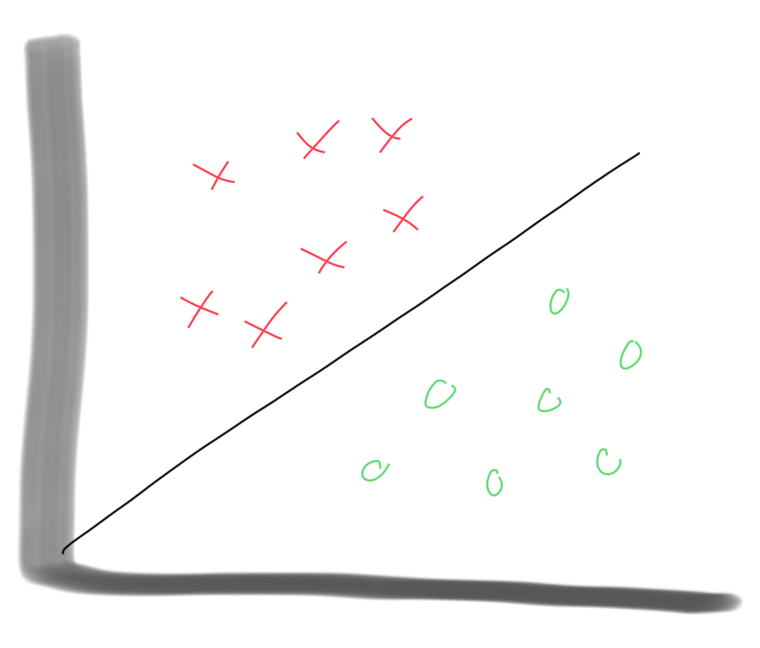
\includegraphics[width=0.5\paperwidth]{../Classification/fig/lin_sep_bn_classes_ipad.jpg}
    \caption{Clear separation between classes.}
    \label{fig:lin-sep-bn-classes}
\end{figure}
Notice the line where our prediction switches from class 1 to class -1. This is precisely where $h(\textbf{x}, \textbf{w}) = 0$, and it is known as the \textbf{decision boundary}.

\begin{definition}{Decision Boundary}{decision-boundary}
	The decision boundary is the line that divides the input space into different target classes. It is learned from an initial data set, and then the target class of new data points can be predicted based on where they fall relative to the decision boundary. At the decision boundary, the discriminant function takes on a value of 0.
\end{definition}

\readernote{You will sometimes see the term \textbf{decision surface} in place of decision boundary, particularly if the input space is larger than two dimensions.}

\subsection{Multiple Classes}
Now consider the case that we have $K > 2$ classes $C_{1}, C_{2}, ..., C_{K}$ to choose between. One obvious approach we might try is to use $K$ different discriminant functions that simply determine whether or not a given input is in that class $C_{k}$. This is known as a \textit{one-versus-all} approach, and it doesn't work properly because we end up with ambiguous regions as demonstrated in Figure \ref{fig:one-vs-all-ambig}.

\begin{figure}
    \centering
    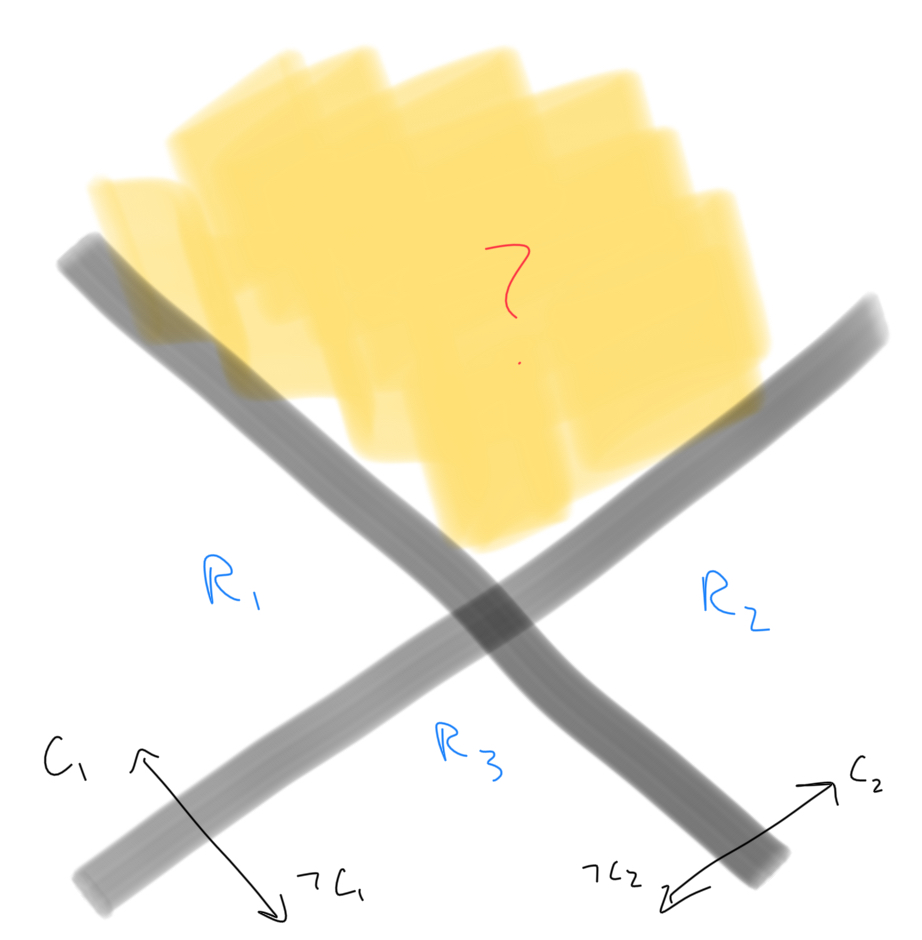
\includegraphics[width=0.5\paperwidth]{../Classification/fig/one_vs_all_ambig_ipad.jpg}
    \caption{Ambiguities arise from one-versus-all method.}
    \label{fig:one-vs-all-ambig}
\end{figure}

Another obvious approach we might employ is to use $\binom{K}{2}$ discriminant functions that each determine whether a given point is more likely to be in class $C_{j}$ or class $C_{k}$. This is known as a \textit{one-versus-one} approach, and it also doesn't work because we again end up with ambiguous regions as demonstrated in Figure \ref{fig:one-vs-one-ambig}.

\begin{figure}
    \centering
    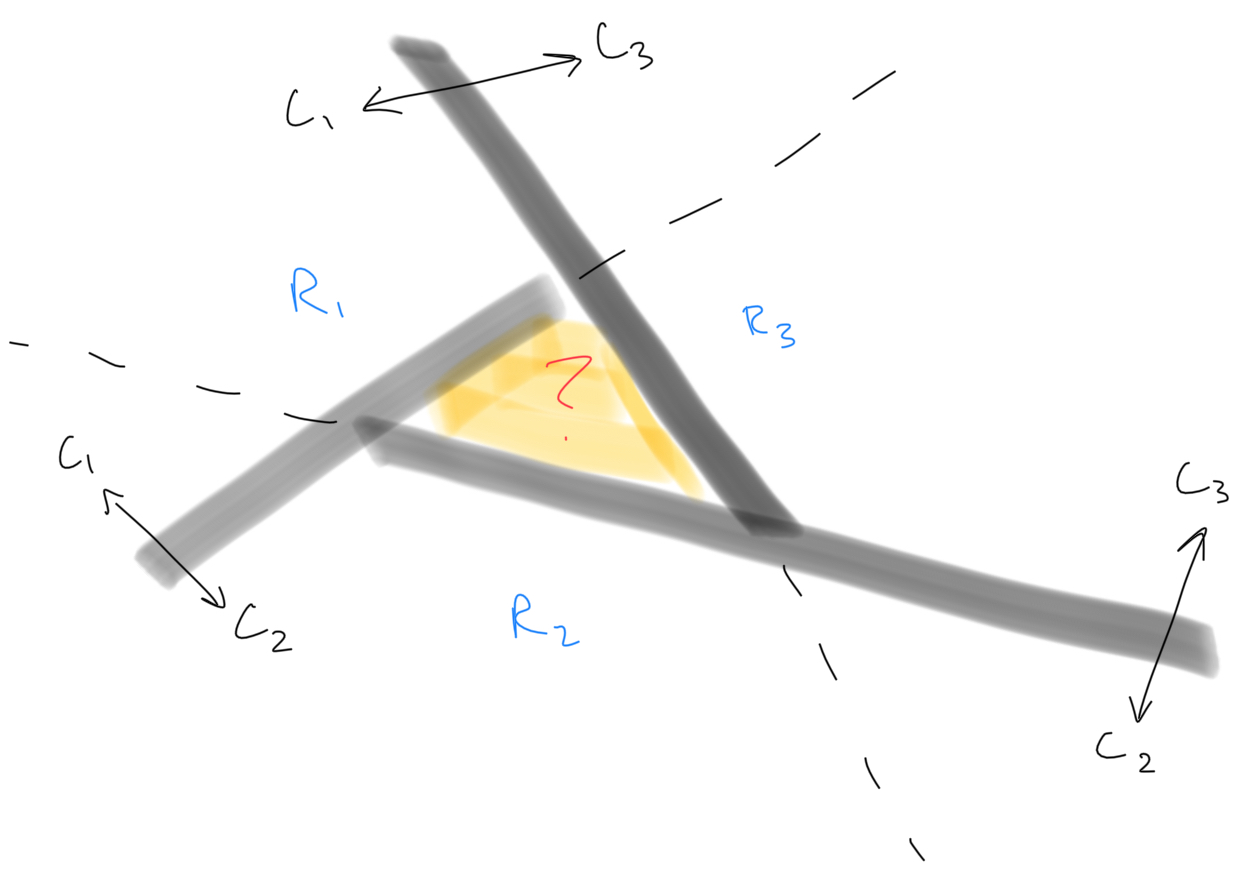
\includegraphics[width=0.5\paperwidth]{../Classification/fig/one_vs_one_ambig_ipad.jpg}
    \caption{Ambiguities arise from one-versus-one method.}
    \label{fig:one-vs-one-ambig}
\end{figure}

Instead, we can avoid these ambiguities in the multi-class case by using $K$ different linear classifiers $h_{k}(\textbf{x}, \textbf{w}_{k})$, and then assigning new data points to the class $C_{k}$ for which $h_{k}(\textbf{x}, \textbf{w}_{k}) > h_{j}(\textbf{x}, \textbf{w}_{j})$ for all $j \neq k$. Then, similar to the two-class case, the decision boundaries are described by the surface along which $h_{k}(\textbf{x}, \textbf{w}_{k}) = h_{j}(\textbf{x}, \textbf{w}_{j})$.

Now that we've explored the multi-class generalization, we can discuss how to learn the weights $w$ that define the optimal discriminant functions.

\subsection{Basis Changes in Classification}
We initially discussed basis changes in the context of linear regression, and they are equally important for classification tasks. For example, consider the data set in Figure \ref{fig:circles-without-basis-change}.

\begin{figure}
    \centering
    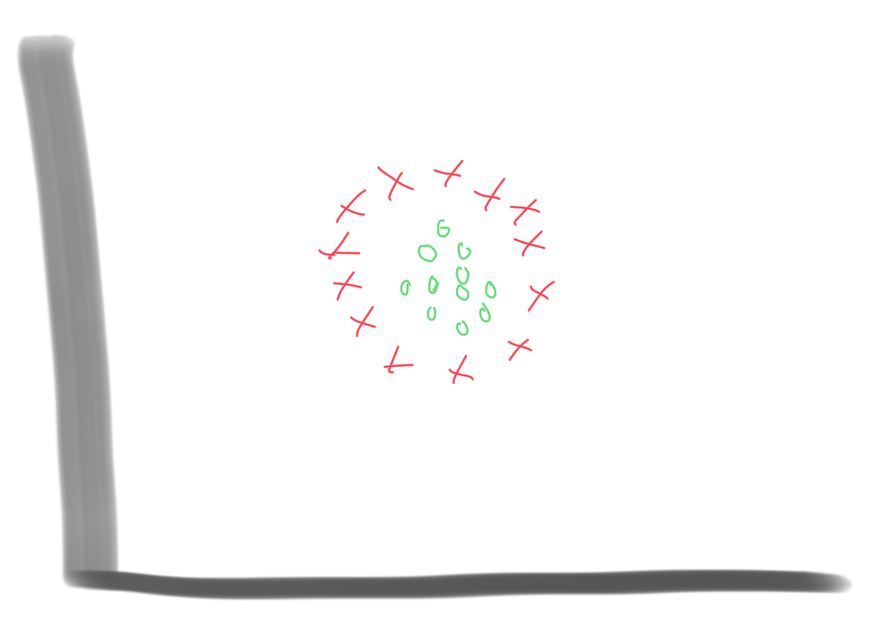
\includegraphics[width=0.5\paperwidth]{../Classification/fig/circles_without_basis_change_ipad.jpg}
    \caption{Data set without any basis functions applied, not linearly separable.}
    \label{fig:circles-without-basis-change}
\end{figure}

It's obviously not possible for us to use a linear classifier to separate this data set. However, if we apply a basis change by squaring one of the data points, we instead have Figure \ref{fig:circles-with-basis-change}, which is now linearly separable by a plane between the two classes.
\begin{figure}
    \centering
    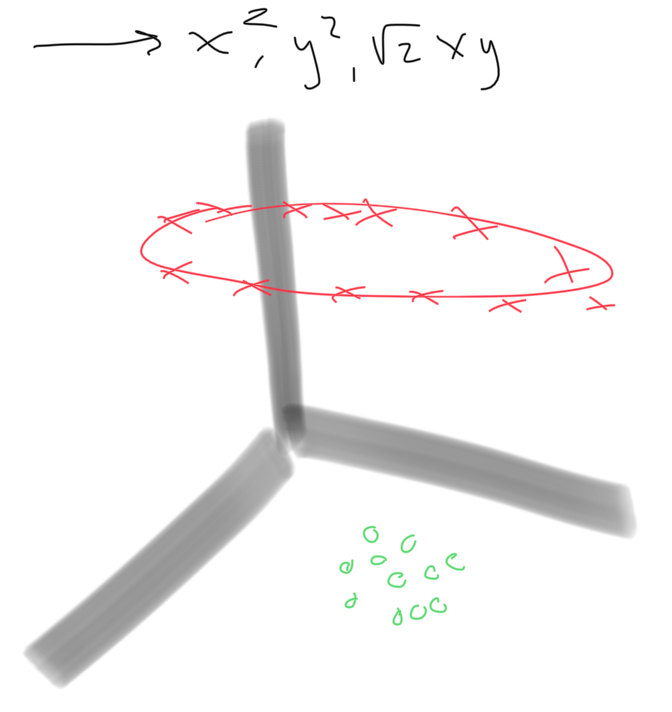
\includegraphics[width=0.5\paperwidth]{../Classification/fig/circles_with_basis_change_ipad.jpg}
    \caption{Data set with basis functions applied, now linearly separable.}
    \label{fig:circles-with-basis-change}
\end{figure}
Applying a generic basis change $\phi(\cdot)$, we can write our generalized linear model as:
\begin{equation} \label{basis-changed-linear-model}
    h_{k}(\textbf{x}, \textbf{w}_{k}) = \textbf{w}_{k}^{T}\phi{(\textbf{x})} = \ \textbf{w}_{k}^{T}\boldsymbol{\phi}
\end{equation}
For the sake of simplicity in the rest of this chapter, we will leave out any basis changes in our derivations, but you should recognize that they could be applied to any of our input data to make the problems more tractable.

\readernote{For an input matrix \textbf{X}, there is a matrix generalization of our basis transformed inputs: $\boldsymbol{\Phi} = \phi(\textbf{X})$, where $\boldsymbol{\Phi}$ is known as the \textit{design matrix}.}

\section{Algorithms for Decision Boundaries}
Now that we have a high-level understanding of what we're trying to accomplish with discriminant functions, we can consider how to solve for the decision boundaries that will dictate our classification decisions. Similar to linear regression, this means we need to establish an objective function to optimize over a training data set. We begin with an objective function that should be familiar from the last chapter: least squares loss.

\subsection{Least Squares Loss}
To find the set of weights \textbf{w} that form the optimal decision boundary between target classes, we will start with a technique that we also used for linear regression: minimizing a least squares loss function.

We first need to introduce the idea of \textit{one-hot encoding}, which simply means that the class of a given data point is described by a vector with $K$ options that has a 1 in the position that corresponds to class $C_{k}$ and 0s everywhere else (note that these classes aren't usually 0-indexed). For example, class $C_{1}$ of 4 classes would be represented by the vector:
\begin{align}
    \begin{bmatrix}
    	1 \\
        0 \\
        0 \\
        0
    \end{bmatrix}
\end{align}
While class $C_{2}$ would be represented by the vector:
\begin{align}
    \begin{bmatrix}
    	0 \\
        1 \\
        0 \\
        0
    \end{bmatrix}
\end{align}
and so on. Now that we have the idea of one-hot encoding, we can describe our target classes for each data point in terms of a one-hot encoded vector, which can then be used in our training process for least squares. \newline \newline
Each class $C_{k}$ gets its own linear function with a different set of weights $\textbf{w}_{k}$:
\begin{align*}
	h_{k}(\textbf{x}, \textbf{w}_{k}) = \textbf{w}_{k}^{T}\textbf{x}
\end{align*}
We can combine the set of weights for each class into a matrix $\textbf{W}$, which gives us our linear classifier:
\begin{equation}
	h(\textbf{x}, \textbf{W}) = \textbf{W}^{T}\textbf{x}
\end{equation}
where each row in the weight matrix \textbf{W} corresponds to the linear function of an individual class. We can use the results derived in the last chapter to find the solution for \textbf{W} that minimizes the least squares loss function. Assuming a data set of input data points $\textbf{X}$ and one-hot encoded target vectors \textbf{Y} (where every row is a single target vector), the optimal solution for \textbf{W} is given by:
\begin{align*}
	\textbf{W}^{*} = (\textbf{X}^{T}\textbf{X})^{-1}\textbf{X}^{T}\textbf{Y}
\end{align*}
which we can then use in our discriminant function $h(\textbf{x}, \textbf{W}^{*})$ to make predictions on new data points.

While least squares gives us an analytic solution for our discriminant function, it also has some significant limitations. For one, least squares penalizes data points that are `too good', meaning they fall too far on the correct side of the decision boundary. Furthermore, it is not robust to outliers, meaning the decision boundary significantly changes with the addition of just a few outlier data points, as seen in Figure \ref{fig:outlier-phenomenon}.

\begin{figure}
    \centering
    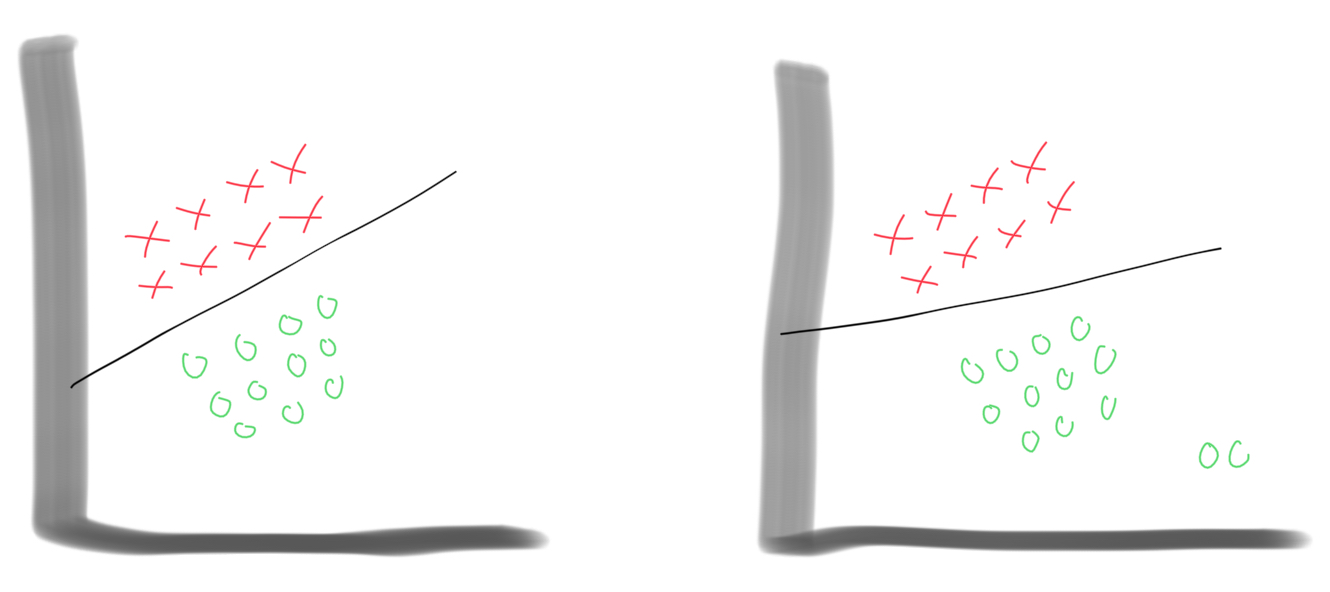
\includegraphics[width=0.5\paperwidth]{../Classification/fig/outlier_phenomenon_ipad.jpg}
    \caption{Outliers significantly impact our decision boundary.}
    \label{fig:outlier-phenomenon}
\end{figure}

We can help remedy the problems with least squares by using alternative methods for solving for our weight parameters.

\subsection{Fisher's Linear Discriminant}
Should we mention this here? Is it necessary?

\subsection{Perceptron Algorithm}
To explain the perceptron algorithm, we must first motivate something called \textbf{0/1 loss}, which is simply an alternative loss function to least squares. The idea behind it is very simple: if we misclassify a point, we incur a loss of 1, and if we classify it correctly, we incur no loss.

While this is a very intuitive loss function, it does not have a closed form solution like least squares does, and it is non-convex so it is not easily optimized. However, the 0/1 loss function inspires a different loss function, known as the \textbf{perceptron loss function}.

The perceptron loss function is a modification of the 0/1 loss function that both provides more fine-grained information and makes it differentiable (which will be important for our ability to optimize our parameters).

To understand the perceptron loss function, it's first necessary to introduce the \textit{rectified linear activation unit}, known as ReLU, seen in Figure \ref{fig:relu-fn}.
\begin{equation}
	\text{ReLU}(z) = \text{max}\{0, z\}
\end{equation}
We can use the form of this function to our advantage in constructing the perceptron loss by recognizing that we wish to incur error when we're wrong (which corresponds to $z > 0$, the right side of the graph that is continuously increasing), and we wish to incur 0 error if we are correct (which corresponds to the left side of the graph where $z < 0$).
\begin{figure}
    \centering
    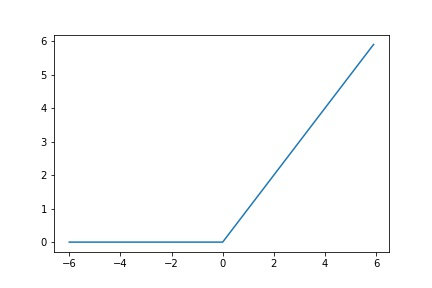
\includegraphics[width=0.5\paperwidth]{../Classification/fig/relu_fn_GEN.jpg}
    \caption{Form of the ReLU function.}
    \label{fig:relu-fn}
\end{figure}

Remember from the previous section on least squares that in the two-class case, we classify a data point $\textbf{x}^{*}$ as being from class 
\textbf{1} if $h(\textbf{x}^{*}, \textbf{w}) \geq 0$, and class \textbf{-1} otherwise. We can combine this logic with ReLU by recognizing that $-h(\textbf{x}^{*}, \textbf{w})y^{*} \geq 0$ when there is a classification error, where $y^{*}$ is the true class of data point $\textbf{x}^{*}$. This has exactly the properties we described above: we incur error when we misclassify, and otherwise we do not incur error. \newline \newline
We can then write the entirety of the perceptron loss function:
\begin{align}
	\mathcal{L}(\textbf{w}) &= \sum_{i=1}^{N} \text{ReLU}(-h(\textbf{x}_{i}, \textbf{w})y_{i}) \\
	&= -\sum_{y_{i} \neq \hat{y}_{i}}^{N} h(\textbf{x}_{i}, \textbf{w})y_{i} \\
	&= -\sum_{y_{i} \neq \hat{y}_{i}}^{N} \textbf{w}^{T}\textbf{x}_{i} y_{i}
\end{align}
where $\hat{y}_{i}$ is our class prediction and $y_{i}$ is the true class value. Notice that misclassified examples contribute positive loss, as desired. We can take the gradient of this loss function, which will allow us to optimize it using stochastic gradient descent. The gradient of the loss with respect to our parameters \textbf{w} is as follows:
\begin{align*}
	\frac{\partial \mathcal{L}(\textbf{w})}{\partial \textbf{w}} = -\sum_{y_{i} \neq \hat{y}_{i}}^{N} \textbf{x}_{i} y_{i}
\end{align*}
and then our update equation from time $t$ to time $t+1$ for a single misclassified example and with learning rate $\eta$ is given by:
\begin{align*}
	\textbf{w}^{(t+1)} = \textbf{w}^{(t)} - \eta\frac{\partial \mathcal{L}(\textbf{w})}{\partial \textbf{w}} = \textbf{w}^{(t)} + \eta \textbf{x}_{i} y_{i}
\end{align*}

There is no need to understand what a learning rate $\eta$ is at the moment, just know for now that it's needed in order to efficiently optimize our parameters $\textbf{w}$. (Should I explain SGD here???) To sum up, the benefits of the perceptron loss function are its differentiability (which allows us to optimize our weight parameters), the fact that it doesn't penalize any correctly classified data points (unlike basic linear classification), and that it penalizes more heavily data points that are more poorly misclassified. Furthermore, the perceptron algorithm guarantees that if there is separability between all of our data points and we run the algorithm for long enough, we will find a setting of parameters that perfectly separates our data set. The proof for this is beyond the scope of this textbook.

\section{Probabilistic Methods}
Unsurprisingly, we can also cast the problem of classification into a probabilistic context, which we now turn our attention to. Within this setting, we have a secondary choice to make between two distinct probabilistic approaches: discriminative or generative. We will explore both of these options.

\subsection{Probabilistic Discriminative Models}
Ultimately, our classification task can be summarized as follows: \textit{given a new data point $\textbf{x}^{*}$, can we accurately predict the target class $y^{*}$?}

Given this problem statement, it makes sense that we might try to model the distribution of $y^{*}|\textbf{x}^{*}$. In fact, modeling this conditional distribution directly is what's known as \textbf{probabilistic discriminative modeling}.

\begin{definition}{Probabilistic Discriminative Modeling}{probabilistic-discriminative-modeling}
    Probabilistic modeling is a classification technique whereby we choose to directly model the conditional class distribution in order to make classification predictions.
\end{definition}

This means that we will start with the functional form of the generalized linear model described by Equation \ref{basis-changed-linear-model}, convert this to a conditional distribution, and then optimize the parameters of the conditional distribution directly using a maximum likelihood procedure. From here, we will be able to make predictions on new data points $\textbf{x}^{*}$. The key feature of this procedure, which is known as \textit{discriminative training}, is that it optimizes the parameters of a conditional distribution directly. We describe a specific, common example of this type of procedure called \textbf{logistic regression} in the next section.

\subsubsection{Logistic Regression}
One problem we need to face in our discriminative modeling paradigm is that the results of our generalized linear model are not probabilities; they are simply real numbers. This is why in the previous paragraph we mentioned needing to convert our generalized linear model to a conditional distribution. That step boils down to somehow squashing the outputs of our generalized linear model onto the real numbers between 0 and 1, which will then correspond to probabilities. To do this, we will apply what is known as the \textbf{logistic sigmoid function}, $\sigma(\cdot)$.

\begin{definition}{Logistic Sigmoid Function, $\sigma(\cdot)$}{logistic-sigmoid-function}
	The logistic sigmoid function is commonly used to compress the real number line down to values between 0 and 1. It is defined functionally as:
	\begin{align*}
		\sigma(z) = \frac{1}{1 + \exp{(-z)}}
	\end{align*}
	As you can see in Figure \ref{fig:log-sig-fn} where the logistic sigmoid function is graphed, it squashes our output domain between 0 and 1 as desired for a probability.
\end{definition}

\begin{figure}
    \centering
    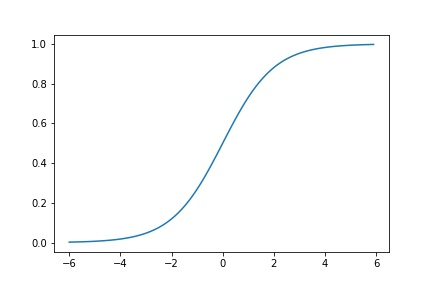
\includegraphics[width=0.5\paperwidth]{../Classification/fig/log_sig_fn_GEN.jpg}
    \caption{Logistic Sigmoid Function.}
    \label{fig:log-sig-fn}
\end{figure}

\readernote{There is a more satisfying derivation for our use of the logistic sigmoid function in logistic regression, but understanding its squashing properties as motivation is sufficient for the purposes of this book.}

Using the logistic sigmoid function, we now have a means of generating a probability that a new data point $\textbf{x}^{*}$ is part of class $y^{*}$. Because we are currently operating in the two-class case, which in this context will be denoted $C_{1}$ and $C_{2}$, we'll write the probability for each of these classes as:
\begin{align*}
	p(y^{*}=C_{1}|\textbf{x}^{*}) &= \sigma(\textbf{w}^{T}\textbf{x}^{*}) \\
	p(y^{*}=C_{2}|\textbf{x}^{*}) &= 1 - p(y^{*}=C_{1}|\textbf{x}^{*})
\end{align*}
Now that we have such functions, we can apply the maximum likelihood procedure to determine the optimal parameters for our logistic regression model.

For a data set \{$\textbf{x}_{i}, y_{i}$\} where $i = 1..N$ and $y_{i} \in \{0,1\}$, the likelihood for our setting of parameters $\textbf{w}$ can be written as:
\begin{equation} \label{log-reg-likelihood}
	p(\{y_{i}\}|\textbf{w}) = \prod_{i=1}^{N} \hat{y}_{i}^{y_{i}} \{1 - \hat{y}_{i}\}^{1 - y_{i}}
\end{equation}
where $\hat{y}_{i} = p(y_{i}=C_{1}|\textbf{x}_{i}) = \sigma(\textbf{w}^{T}\textbf{x}_{i})$.

In general, we would like to maximize this probability to find the optimal setting of our parameters. This is exactly what we intend to do, but with two further simplifications. First, we're going to maximize the probability of the \textit{logarithm} of the likelihood. As a monotonically increasing function, maximizing the logarithm of the likelihood (called the \textit{log likelihood}) will result in the same optimal setting of parameters as if we had just optimized the likelihood directly. Furthermore, using the log likelihood has the nice effect of turning what is currently a product of terms from $1..N$ to a sum of terms from $1..N$, which will make our calculations nicer. Second, we will turn our log likelihood into an \textit{error function} by taking the negative of our log likelihood expression. Now, instead of maximizing the log likelihood, we will be minimizing the error function, which will again find us the same setting of parameters.

\readernote{It's worth rereading the above paragraph again to understand the pattern presented there, which we will see several times throughout this book. Instead of maximizing a likelihood function directly, it is often easier to define an error function using the negative log likelihood, which we can then minimize to find the optimal setting of parameters for our model.}

After taking the negative logarithm of the likelihood function defined by Equation \ref{log-reg-likelihood}, we are left with the following term, known as the \textit{cross-entropy error function}, which we will seek to minimize:
\begin{equation} \label{cross-entropy-error-fn}
	\mathrm{E}(\textbf{w}) = - \ln{p(\{y_{i}\}|\textbf{w})} = - \sum_{i=1}^{N} \{y_{i}\ln{\hat{y}_i} + (1 - y_{i})\ln{(1-\hat{y_{i}})}\}
\end{equation}
where as before $\hat{y}_{i} = p(y_{i}=C_{1}|\textbf{x}_{i}) = \sigma(\textbf{w}^{T}\textbf{x}_{i})$. Now, to solve for the optimal setting of parameters using a maximum likelihood approach as we've done previously, we start by taking the gradient of the cross-entropy error function with respect to \textbf{w}:
\begin{equation} \label{log-reg-gradient}
	\nabla \mathrm{E}(\textbf{w}) = \sum_{i=1}^{N}(\hat{y}_{i} - y_{i})\textbf{x}_{i}
\end{equation}
which we arrive at by recognizing that the derivative of the logistic sigmoid function can be written in terms of itself as:
\begin{align*}
	\frac{\partial \sigma(z)}{\partial z} = \sigma(z)(1 - \sigma(z))
\end{align*}
(I can include the derivation if that's helpful, thoughts???) Let's inspect the form of Equation \ref{log-reg-gradient} for a moment to understand its implications. First, it's a summation over all of our data points, as we would expect. Then, for each data point, we are taking the difference between our predicted value $\hat{y}_{i}$ and the actual value $y_{i}$, and multiplying that difference by the input vector $\textbf{x}_{i}$.

While a closed form solution does not present itself here as it did in the case of linear regression due to the nonlinearity of the logistic sigmoid function, we can still optimize the parameters \textbf{w} of our model using an iterative procedure that updates our parameters by moving toward the minimum of the error function defined in Equation \ref{cross-entropy-error-fn}.

\subsubsection{Multi-Class Logistic Regression and Softmax}
As we saw when working with discriminant functions, we also need to account for multi-class problems, which are practically speaking more common than the simple two-class scenario.

In the logistic regression setting (which is a form of \textit{discriminative modeling}, not to be confused with \textit{discriminant functions}), we are now working with probabilities, which is why we introduced the `probability squashing' sigmoidal function $\sigma(\cdot)$. Note that the sigmoidal function is also sometimes known as the sigmoidal activation function.

Similarly, in the multi-class logistic regression setting, we would like to also have a probability squashing function that generalizes beyond two classes. This generalization of the sigmoidal function is known as \textbf{softmax}.

\begin{definition}{Softmax}{softmax}
Softmax is the multi-class generalization of the sigmoidal activation function. It accepts a vector of activations (inputs) and returns a vector of probabilities corresponding to those activations. It is defined as follows:
\begin{align*}
	\text{softmax}_{k}(\textbf{z}) = \frac{\exp{(z_{k})}}{\sum_{i=1}^{K} \exp{(z_{i})}}\text{, for all $k$}
\end{align*}
\end{definition}

Multi-class logistic regression uses softmax over a vector of activations to select the most likely target class for a new data point. It does this by applying softmax and then assigning the new data point to the class with the highest probability.

\begin{example}{Softmax Example}{softmax-example}
	Consider an example that has three classes: $C_{1}, C_{2}, C_{3}$. Let's say we have an activation vector \textbf{z} for our new data point $\textbf{x}$ that we wish to classify, given by:
	\begin{align*}
		\textbf{z} = \textbf{W}^{T}\textbf{x} =
			\begin{bmatrix}
		    	4 \\
		        1 \\
		        7
		    \end{bmatrix}
	\end{align*}
	where
	\begin{align*}
		\textbf{z}_{j} = \textbf{w}_{j}^{T}\textbf{x}
	\end{align*}
	Then, using our definition of softmax, we have:
	\begin{align*}
		\text{softmax}(\textbf{z}) =
			\begin{bmatrix}
				0.047 \\
				0.002 \\
				0.950
		    \end{bmatrix}
	\end{align*}
	And therefore, we would assign our new data point $\textbf{x}$ to class $C_{3}$, which has the largest activation.
\end{example}

As in the two-class logistic regression case, we now need to solve for the parameters \textbf{W} of our model, also written as \{$\textbf{w}_{j}$\}. Assume we have an observed data set \{$\textbf{x}_{i}, \textbf{y}_{i}$\} for $i=1..N$ where $\textbf{y}_{i}$ are one-hot encoded target vectors.  We begin this process by writing the likelihood for our data, which is only slightly modified here to account for multiple classes:

\begin{equation} \label{multi-class-log-reg-likelihood}
	p(\{\textbf{y}_{i}\}|\textbf{W}) = \prod_{i=1}^{N}\prod_{j=1}^{K} p(\textbf{y}_{i}=C_{k}|\textbf{x}_{i})^{y_{ij}} = \prod_{i=1}^{N}\prod_{j=1}^{K} \hat{y}_{ij}^{y_{ij}}
\end{equation}
where $\hat{y}_{ij} = \text{softmax}_{j}(\textbf{W}\textbf{x}_{i})$ \newline

We can now take the negative logarithm to get the cross-entropy error function for the multi-class classification problem:
\begin{equation} \label{multi-class-cross-entropy-error-fn}
	\mathrm{E}(\textbf{W}) = - \ln{p(\{\textbf{y}_{i}\}|\textbf{W})} = - \sum_{i=1}^{N}\sum_{j=1}^{K} y_{ij} \ln{\hat{y}_{ij}}
\end{equation}
As in the two-class case, we now take the gradient with respect to one of our weight parameter vectors $\textbf{w}_{j}$:
\begin{equation} \label{multi-class-log-reg-gradient}
	\nabla_{\textbf{w}_{j}} \mathrm{E}(\textbf{W}) = \sum_{i=1}^{N}(\hat{y}_{ij} - y_{ij})\textbf{x}_{i}
\end{equation}
which we arrived at by recognizing that the derivative of the softmax function with respect to the input activations $z_{j}$ can be written in terms of itself:
\begin{align*}
	\frac{\partial \text{softmax}_{k}(z)}{\partial z_{j}} = \text{softmax}_{k}(z)(\mathrm{I}_{kj} - \text{softmax}_{j}(z))
\end{align*}
where $\mathrm{I}$ is the identity matrix.

As in the two-class case, now that we have this gradient expression, we can use an iterative procedure to update our parameters $\textbf{W}$ toward their optimal values by minimizing the error function.

\subsection{Probabilistic Generative Models}
With the probabilistic discriminative modeling approach, we elected to directly model the class-conditional probability $y^{*}|\textbf{x}^{*}$. However, there was an alternative option: we could have instead modeled the joint distribution of the class $y^{*}$ and the input data point $\textbf{x}^{*}$ together as $p(y^{*}, \textbf{x}^{*})$. This approach is what's known as \textbf{probabilistic generative modeling} because we actually model the process by which the data was generated.

To model the data generating process in classification tasks generally acknowledges that a data point is produced by first selecting a class $y^{*}$ from a categorical class prior $p(y^{*})$ and then generating the data point $\textbf{x}^{*}$ itself from the class-conditional distribution $p(y^{*}|\textbf{x}^{*})$, the form of which is problem specific.

\readernote{Notice that with probabilistic generative modeling, we choose a specific distribution for our class-conditional densities instead of simply using a generalized linear model combined with a sigmoid/softmax function as we did in the logistic regression setting. This highlights the difference between discriminative and generative modeling: in the generative setting, we are modeling the production of the data itself instead of simply optimizing the parameters of a more general model that predicts class membership directly.}

\subsubsection{Classification in the Generative Setting}
Now that we're situated in the generative setting, we turn our attention to the actual problem of using our model to predict class membership of new data points $\textbf{x}^{*}$.

To perform classification, we will pick the class $C_{k}$ that maximizes the probability of $\textbf{x}^{*}$ being from that class as defined by $p(y^{*} = C_{k} | \textbf{x}^{*})$. We can relate this conditional density to the joint density $p(y^{*}, \textbf{x}^{*})$ through Bayes' Rule:
\begin{align*}
	p(y^{*} = C_{k} | \textbf{x}^{*}) = \frac{p(y^{*}, \textbf{x}^{*})}{p(\textbf{x}^{*})} = \frac{p(\textbf{x}^{*} | y^{*} = C_{k})p(y^{*} = C_{k})}{p(\textbf{x}^{*})} \propto p(\textbf{x}^{*} | y^{*} = C_{k})p(y^{*} = C_{k})
\end{align*}
where $p(\textbf{x}^{*})$ is a constant that can be ignored as it will be the same for every conditional probability $p(y^{*} = C_{k}|\textbf{x}^{*})$.

Recall that the class prior $p(y)$ will always be a categorical distribution (the multi-class generalization of the Bernoulli distribution), while the class-conditional distribution can be specified using prior knowledge of the problem domain. Once we have specified this class conditional distribution, we can solve for the parameters of both that model and the categorical distribution using a maximum likelihood procedure.

\subsubsection{Maximum Likelihood Solution}
We're going to derive the maximum likelihood solution for the parameters of our probabilistic generative model in the two-class setting, allowing that the multi-class generalization will be a straightforward exercise.

Let's start by assuming a Gaussian conditional distribution for our data $p(\textbf{x} | y = C_{k})$. Given a data set \{$\textbf{x}_{i}, y_{i}$\} for $i = 1..N$, where $y_{i} = 1$ corresponds to class $C_{1}$ and $y_{i} = 0$ corresponds to class $C_{2}$, we can construct our maximum likelihood solution. Let's first specify our class priors:
\begin{align*}
	p(C_{1}) &= \pi \\
	p(C_{2}) &= 1 - \pi
\end{align*}
For simplicity, we'll assume a shared covariance matrix $\boldsymbol{\Sigma}$ between our two classes. Then, for data points $\textbf{x}_{i}$ from class $C_{1}$, we have:
\begin{align*}
	p(\textbf{x}_{i}, C_{1}) = p(C_{1})p(\textbf{x}_{i}|C_{1}) = \pi\mathcal{N}(\textbf{x}_{i} | \boldsymbol{\mu}_{1}, \boldsymbol{\Sigma})
\end{align*}
And for data points $\textbf{x}_{i}$ from class $C_{2}$, we have:
\begin{align*}
	p(\textbf{x}_{i}, C_{2}) = p(C_{2})p(\textbf{x}_{i}|C_{2}) = (1-\pi)\mathcal{N}(\textbf{x}_{i} | \boldsymbol{\mu}_{2}, \boldsymbol{\Sigma})
\end{align*}
Using these two densities, we can construct our likelihood function:
\begin{align*}
	\mathcal{L}(\pi, \boldsymbol{\mu}_{1}, \boldsymbol{\mu}_{2}, \boldsymbol{\Sigma}) = \prod_{i=1}^{N} \bigg( \pi\mathcal{N}(\textbf{x}_{i} | \boldsymbol{\mu}_{1}, \boldsymbol{\Sigma}) \bigg)^{y_{i}} \bigg( (1-\pi)\mathcal{N}(\textbf{x}_{i} | \boldsymbol{\mu}_{2}, \boldsymbol{\Sigma}) \bigg)^{1 - y_{i}}
\end{align*}
As usual, we will take the logarithm which is easier to work with:
\begin{align*}
	\ln \mathcal{L}(\pi, \boldsymbol{\mu}_{1}, \boldsymbol{\mu}_{2}, \boldsymbol{\Sigma}) = \sum_{i=1}^{N} y_{i} \ln \bigg( \pi\mathcal{N}(\textbf{x}_{i} | \boldsymbol{\mu}_{1}, \boldsymbol{\Sigma}) \bigg) + (1 - y_{i}) \ln \bigg( (1-\pi)\mathcal{N}(\textbf{x}_{i} | \boldsymbol{\mu}_{2}, \boldsymbol{\Sigma}) \bigg)
\end{align*}
We can now optimize for our parameters $\pi, \boldsymbol{\mu}_{1}, \boldsymbol{\mu}_{2}, \text{and}, \boldsymbol{\Sigma}$ separately, using the usual procedure of taking the derivative, setting equal to 0, and then solving for the parameter of interest.

\begin{derivation}{MLE Solution}{mle-solution-derivation}
    Beginning with $\pi$, we'll concern ourselves only with the terms that depend on $\pi$ which are:
    \begin{align*}
    	\sum_{i=1}^{N} y_{i}\ln{\pi} + (1-y_{i})\ln{(1 - \pi)}
    \end{align*}
    Taking the derivative with respect to $\pi$, setting equal to 0, rearranging, we get:
    \begin{align*}
    	\pi = \frac{1}{N} \sum_{i=1}^{N} y_{i} = \frac{N_{1}}{N} = \frac{N_{1}}{N_{1} + N_{2}}
    \end{align*}
    where $N_{1}$ is the number of data points in our data set from class $C_{1}$, $N_{2}$ is the number of data points from class $C_{2}$, and $N$ is just the total number of data points. This means that the maximum likelihood solution for $\pi$ is the fraction of points that are assigned to class $C_{1}$, a fairly intuitive solution and one that will be commonly seen when working with maximum likelihood calculations.

    Let's now perform the maximization for $\boldsymbol{\mu}_{1}$. Start by considering the terms from our log likelihood involving $\boldsymbol{\mu}_{1}$:
    \begin{align*}
    	\sum_{i=1}^{N} y_{i} \ln \mathcal{N}(\textbf{x}_{i} | \boldsymbol{\mu}_{1}, \boldsymbol{\Sigma}) = -\frac{1}{2} \sum_{i=1}^{N} y_{i} (\textbf{x}_{i} - \boldsymbol{\mu}_{1})^{T}\boldsymbol{\Sigma}^{-1}(\textbf{x}_{i} - \boldsymbol{\mu}_{1}) + c
    \end{align*}
    where $c$ are constants not involving the $\boldsymbol{\mu}_{1}$ term. Taking the derivative with respect to $\boldsymbol{\mu}_{1}$, setting equal to 0, and rearranging:
    \begin{align*}
    	\boldsymbol{\mu}_{1} = \frac{1}{N_{1}} \sum_{i=1}^{N} y_{i}\textbf{x}_{i}
    \end{align*}
    which is simply the average of all the data points $\textbf{x}_{i}$ assigned to class $C_{1}$, a very intuitive result. By the same derivation, the maximum likelihood solution for $\boldsymbol{\mu}_{2}$ is:
    \begin{align*}
    	\boldsymbol{\mu}_{2} = \frac{1}{N_{2}} \sum_{i=1}^{N} (1-y_{i})\textbf{x}_{i}
    \end{align*}

    And finally, we can derive the maximum likelihood solution for the shared covariance matrix $\boldsymbol{\Sigma}$. Start by considering the terms in our log likelihood expression involving $\boldsymbol{\Sigma}$:
    \begin{align*}
    	-\frac{1}{2} \sum_{i=1}^{N} y_{i} \ln{|\boldsymbol{\Sigma}|} -\frac{1}{2} \sum_{i=1}^{N} y_{i} (\textbf{x}_{i} - \boldsymbol{\mu}_{1})^{T}\boldsymbol{\Sigma}^{-1}(\textbf{x}_{i} - \boldsymbol{\mu}_{1}) -\frac{1}{2} \sum_{i=1}^{N} (1-y_{i}) \ln{|\boldsymbol{\Sigma}|} -\frac{1}{2} \sum_{i=1}^{N} (1-y_{i}) (\textbf{x}_{i} - \boldsymbol{\mu}_{2})^{T}\boldsymbol{\Sigma}^{-1}(\textbf{x}_{i} - \boldsymbol{\mu}_{2})
    \end{align*}
    Taking the derivative with respect to $\boldsymbol{\Sigma}$:
    \begin{align*}
    	N\boldsymbol{\Sigma}^{-T} - \frac{1}{2}\sum_{i=1}^{N} y_{i} \boldsymbol{\Sigma}^{-T}(\textbf{x}_{i} - \boldsymbol{\mu}_{1})(\textbf{x}_{i} - \boldsymbol{\mu}_{1})^{T}\boldsymbol{\Sigma}^{-T} - \frac{1}{2}\sum_{i=1}^{N} (1-y_{i}) \boldsymbol{\Sigma}^{-T}(\textbf{x}_{i} - \boldsymbol{\mu}_{2})(\textbf{x}_{i} - \boldsymbol{\mu}_{2})^{T}\boldsymbol{\Sigma}^{-T}
    \end{align*}
    Setting equal to 0 and rearranging to solve for $\boldsymbol{\Sigma}$:
    \begin{align*}
    	\boldsymbol{\Sigma} = \frac{1}{N} \sum_{i=1}^{N} \bigg( y_{i}(\textbf{x}_{i} - \boldsymbol{\mu}_{1})(\textbf{x}_{i} - \boldsymbol{\mu}_{1})^{T} + (1-y_{i})(\textbf{x}_{i} - \boldsymbol{\mu}_{2})(\textbf{x}_{i} - \boldsymbol{\mu}_{2})^{T} \bigg)
    \end{align*}
    which has the intuitive interpretation that the maximum likelihood solution for the shared covariance matrix is the weighted average of the two individual covariance matrices.
\end{derivation} \newpage

It is relatively straightforward to extend these maximum likelihood derivations from their two-class form to their more general, multi-class form.

\subsubsection{Naive Bayes}
There exists a further simplification to probabilistic generative modeling known as \textbf{Naive Bayes}.

\begin{definition}{Naive Bayes}{naive-bayes-definition}
	Naive Bayes is a type of generative model for classification tasks. It imposes the simplifying rule that for a given class $C_{k}$, we assume that each feature of the data points $\textbf{x}$ generated within that class are independent (hence the descriptor `naive'). This means that the conditional distribution $p(\textbf{x} | y = C_{k})$ can be written as:
	\begin{align*}
		p(\textbf{x} | y = C_{k}) = \prod_{i = 1}^{D} p(x_{j} | y = C_{k})
	\end{align*}
	where $D$ is the number of features in our data point $\textbf{x}$ and $C_{k}$ is the class. Note that Naive Bayes does not specify the form of the model $p(x_{j} | y = C_{k})$, this decision is left up to us.
\end{definition}
This is obviously not a realistic simplification for all scenarios, but it can make our calculations easier and may actually hold true in certain cases. We can build more intuition for how Naive Bayes works through an example.

\begin{example}{Naive Bayes Example}{naive-bayes-example}
	Suppose you are given a biased two-sided coin and two biased dice. The coin has probabilities as follows:
	\begin{align*}
		\textbf{Heads}: 30\% \\
		\textbf{Tails}: 70\%
	\end{align*}
	The dice have the numbers 1 through 6 on them, but they are biased differently. Die 1 has probabilities as follows:
	\begin{align*}
		\textbf{1}: 40\% \\
		\textbf{2}: 20\% \\
		\textbf{3}: 10\% \\
		\textbf{4}: 10\% \\
		\textbf{5}: 10\% \\
		\textbf{6}: 10\%
	\end{align*}
	Die 2 has probabilities as follows:
	\begin{align*}
		\textbf{1}: 20\% \\
		\textbf{2}: 20\% \\
		\textbf{3}: 10\% \\
		\textbf{4}: 30\% \\
		\textbf{5}: 10\% \\
		\textbf{6}: 10\%
	\end{align*}
	Your friend is tasked with doing the following. First, they flip the coin. If it lands Heads, they select Die 1, otherwise they select Die 2. Then, they roll that die 10 times in a row, recording the results of the die rolls. After they have completed this, you get to observe the aggregated results from the die rolls. Using this information (and assuming you know the biases associated with the coin and dice), you must then classify which die the rolls came from. Assume your friend went through this procedure and produced the following counts:
	\begin{align*}
		\textbf{1}: 3 \\
		\textbf{2}: 1 \\
		\textbf{3}: 2 \\
		\textbf{4}: 2 \\
		\textbf{5}: 1 \\
		\textbf{6}: 1
	\end{align*}
	Determine which die this roll count most likely came from. \newline \newline

	\textbf{Solution:} \newline
	This problem is situated in the Naive Bayes framework: for a given class (dictated by the coin flip), the outcomes within that class (die rolls) are independent. Making a classification in this situation is as simple as computing the probability that the selected die produced the given roll counts. Let's start by computing the probability for Die 1:
	\begin{align*}
		p(\text{Die 1}) &= p(\text{Coin Flip = Heads}) * p(\text{Roll Count = }[3,1,2,2,1,1]) \\
		&\propto 0.3 * (0.4)^{3} * (0.2)^{1} * (0.1)^{2} * (0.1)^{2} * (0.1)^{1} * (0.1)^{1} \\
		&\propto 3.84 * 10^{-9}
	\end{align*}
	Notice that we don't concern ourselves with the normalization constant for the probability of the roll count - this will not differ between the choice of dice and we can thus ignore it for simplicity. Now the probability for Die 2:
	\begin{align*}
		p(\text{Die 2}) &= p(\text{Coin Flip = Tails}) * p(\text{Roll Count = }[3,1,2,2,1,1]) \\
		&\propto 0.7 * (0.2)^{3} * (0.2)^{1} * (0.1)^{2} * (0.3)^{2} * (0.1)^{1} * (0.1)^{1} \\
		&\propto 1.008 * 10^{-8}
	\end{align*}
	Therefore, we would classify this roll count as having come from Die 2. \newline \newline
	Note that this problem asked us only to make a classification prediction after we already knew the parameters governing the coin flip and dice rolls. However, given a data set, we could have also used a maximum likelihood procedure under the Naive Bayes assumption to estimate the values of the parameters governing the probability of the coin flip and die rolls.
\end{example}

\section{Conclusion}
In this chapter, we looked at different techniques for solving classification problems, including discriminant functions, probabilistic discriminative models, and probabilistic generative models. In particular, we emphasized the distinction between two-class and multi-class problems as well as the philosophical differences between generative and discriminative modeling.

We also covered several topics that we will make use of in subsequent chapters, including sigmoid functions and softmax, maximum likelihood solutions, and further use of basis changes.

By now, you have a sound understanding of generative modeling and how it can be applied to classification tasks. In the next chapter, we will explore how generative modeling is applied to a still broader class of problems.

\section{Practice Problems}
\begin{enumerate}
    \item Small toy example of solving for optimal weights for discriminant functions.
    \item Demonstrate that least squares penalizes points that are `too good'.
    \item One update step of the perceptron algorithm.
    \item Using softmax.
    \item Naive Bayes problem - estimating the parameters given a data set derivation.
    \item Maximum likelihood estimation for probabilistic generative models in the multi-class setting.
    \item Using probabilistic discriminative modeling and probabilistic generative modeling to make predictions on a small data set.
\end{enumerate}